\section{Lie Groups}

Historically and in practice, Lie groups arise first as the study of the transformation of geometric objects.
Let us consider the example of a sphere in euclidean space.
There are in a sense three ways to rotate a sphere.
Choose a point on the equator of a sphere.
You can rotate the sphere so that this point moves towards a pole (y-axis rotation), so that this point moves along the equator (z-axis rotation), or so that the point is stationary (x-axis rotation).
Moreover these rotations are continuous in a way that rotating an equilateral triangle is not, because at each stage of rotation the sphere as a whole occupies the same space.

How should we describe the rotations of a sphere?
First observe that antipodal points remain antipodal, so the rotation of a sphere extends to a linear transformation of $\bbR^3$.
Hence any rotation $R$ can be described by a real $3\times 3$-matrix.
Moreover rotation is length and angle preserving, so $\langle Rx, Ry \rangle = \langle x, y \rangle$.
This holds exactly if $R^TR = I$, which gives us the orthogonal group
\[
\O(3) = \{ R \in \Mat(3,\bbR) \mid R^TR = I \}.
\]
We can understand the defining equation as saying that the columns of $R$ are an orthonormal basis of $\bbR^3$.
Indeed they are the images of the standard basis of $\bbR^3$ under $R$.
We were discussing proper rotations, which are by definition orientation preserving, so we want that the columns of $R$ are a right handed basis.
That leads to the special orthogonal group
\[
\SO(3) = \{ R \in \O(3) \mid \det R = 1 \}.
\]
The group operation is composition of operators, ie matrix multiplication.
Both groups clearly contain the identity $I$.
The property $R^T R = I$ implies $(\det R)^2 = 1$, so these are invertible matrices.
Therefore they really are groups.
Moreover the sign of the determinant can be used to distinguish a proper rotation from an improper one.
% The later group are the (proper) rotations, the former is a group that includes reflections.

Heuristically, we have nine choices for the matrix of $R$ subject to the restriction each of the three columns must be unit length and the restriction that pairs of columns must be orthogonal (six restrictions total).
This agrees with the three degrees of freedom we argued for above.
To see this is a manifold however we consider a function $f$ from $\Mat(3,\bbR)$ to the symmetric matrices given by $f(R) = R^TR$.
The orthogonal matrices are exactly $\O(3) = f^{-1}(I)$.
The derivative at $R$ in the direction $S$ is $f'(R)(S) = R^TS + S^T R = R^T S + (R^T S)^T$.
At a point $R \in \O(3)$ this is surjective in $S$: for any symmetric matrix $Y$ let $S = \frac{1}{2}RY$.
Hence $f$ is full rank at every point $R \in \O(3)$ and by the implicit function theorem $\O(3)$ is an embedded submanifold of $\Mat(3,\bbR) \cong \bbR^9$.
The symmetric matrices are dimension $6$, so in fact our heuristic has been formalised to a rigorous argument.

The group operation, matrix multiplication, is a smooth operation on the set of matrices because it is polynomial.
Therefore it is also smooth when restricted to an embedded submanifold.
Similarly inversion is an everywhere defined rational function on the open set of invertible matrices, so also smooth on $\O(3)$.
This makes $\O(3)$ and $\SO(3)$ Lie groups.

Now that we know that $\O(3)$ is a manifold, we can ask about its connected components.
Intuitively we can rotate any right handed frame $R \in \SO(3)$ to the standard basis $I$, so $\SO(3)$ is connected.
Because it contains the identity, it is called the identity component.
On the other hand, the reflection in the plane $x_1 = 0$ has determinant $-1$ whereas $\det I = 1$.
Determinant is continuous (polynomial) function on matrices and as already noted $R \in \O(3)$ implies $\det R = \pm 1$, so this reflection is not in the identity component.
Composing an improper rotation with this reflection gives a proper rotation and vice-versa. Therefore the subset of $\O(3)$ with $\det R = -1$ is also a connected component of $\O(3)$.
In conclusion, $\SO(3)$ is connected and $\O(3)$ has two diffeomorphic components.

To understand the topology of $\SO(3)$ an alternate description is useful.
Every rotation of $\bbR^3$ is rotation around an axis.
More precisely, we can describe the rotation axis by a unit vector $u$ such that the rotation is right handed by an angle $\theta$ in the range $[0,\pi]$.
Thus the rotations can be described by the closed unit ball $\theta u \in \overline{B(0,1)}$.
The origin is rotation by angle $0$ with the axis of rotation irrelevant.
But similarly, rotation by $\pi$ around $u$ and $-u$ are the same rotation.
Thus $\SO(3)$ can be modelled as the closed unit ball with antipodal points on the boundary identified, the real projective space $\RP^3$.

In this model it is easy to understand the fundamental group.
Take any closed loop in $\SO(3)$.
If it lies entirely in $B(0,1)$ then it can be contracted to a point.
% If it meets $\partial B(0,1)$ in one point then we may describe it as a path $\gamma : (0,1) \to B(0,1)$ with $\gamma(1) = - \gamma(0) \in \partial B(0,1)$. 
Otherwise it can be divided into a collection of segments $\gamma_i : (0,1) \to B(0,1)$ with $\gamma_{i+1}(0) = \pm \gamma_i(1) \in \partial B(0,1)$ and $\gamma_1(0) = \pm \gamma_n(1) \in \partial B(0,1)$.
These conditions ensure that the segments connect up to a loop in $\RP^3$.
We call the number of negative signs the index of the loop.
If $\gamma_{i+1}(0) = \gamma_i(1)$ then it is possible to move this point into the interior of $B(0,1)$ and fuse these two segments together into a single segment.
This doesn't change the index of the loop.
As an extreme case, if the index is zero, then we can move all the endpoints of the segments off $\partial B(0,1)$ and contract the loop to a point.
So without loss of generality, assume that all the signs are negatives.
\begin{center}
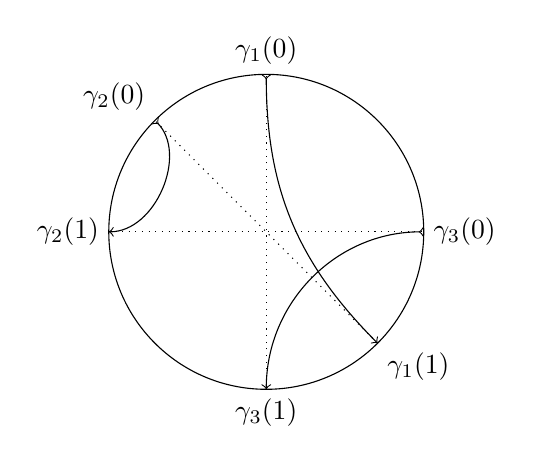
\begin{tikzpicture}
    % Circle
    \draw (0,0) circle (2cm);
    
    % Curve 1
    \draw[>->] (90:2cm) to[out=270, in=135] (-45:2cm);
    \node at (90:2cm) [above] {$\gamma_1(0)$};
    \node at (-45:2cm) [below right] {$\gamma_1(1)$};

    \draw[dotted] (-45:2cm) -- (135:2cm);
    
    % Curve 2
    \draw[>->] (135:2cm) to[out=-45, in=0] (180:2cm);
    \node at (135:2cm) [above left] {$\gamma_2(0)$};
    \node at (180:2cm) [left] {$\gamma_2(1)$};

    \draw[dotted] (180:2cm) -- (0:2cm);

    % Curve 3
    \draw[>->] (0:2cm) to[out=180, in=90] (-90:2cm);
    \node at (0:2cm) [right] {$\gamma_3(0)$};
    \node at (-90:2cm) [below] {$\gamma_3(1)$};

    \draw[dotted] (-90:2cm) -- (90:2cm);
\end{tikzpicture}
\begin{tikzpicture}
    % Circle
    \draw (0,0) circle (2cm);
    
    % Curve 1
    \draw[>->] (90:2cm) to[out=270, in=110] (0:2cm);
    \node at (90:2cm) [above] {$\gamma_1(0)$};
    % \node at (-45:2cm) [below right] {$\gamma_1(1)$};

    % \draw[dotted] (-45:2cm) -- (135:2cm);
    
    % Curve 2
    \draw[>->] (180:2cm) to[out=45, in=180] (150:1.5cm) to[out=0, in=0]  (180:2cm);
    % \node at (135:2cm) [above left] {$\gamma_2(0)$};
    \node at (180:2cm) [left] {$\gamma_2(0) = \gamma_2(1)$};

    \draw[dotted] (180:2cm) -- (0:2cm);

    % Curve 3
    \draw[>->] (0:2cm) to[out=180, in=90] (-90:2cm);
    \node at (0:2cm) [right] {$\gamma_1(1)=\gamma_3(0)$};
    \node at (-90:2cm) [below] {$\gamma_3(1)$};

    \draw[dotted] (-90:2cm) -- (90:2cm);
\end{tikzpicture}
\end{center}
If there is more than one segment, we can move $\gamma_1$ and $\gamma_2$ such that $\gamma_1(0)$ and $\gamma_2(1)$ remain fixed (so no other segments are affected) but $\gamma_2(0)$ is moved to $\gamma_2(1)$ (so necessarily $\gamma_1(1) \to - \gamma_2(1)$).
Then $\gamma_2$ can be contracted to the constant map $\gamma_1(1) = -\gamma_2(0) = -\gamma_2(1) = \gamma_3(0)$.
This means that we can eliminate $\gamma_2$ and fuse $\gamma_1$ and $\gamma_3$ into a single segment.
In particular, the index has decreased by two.
This argument has not quite proved that the parity of the index (even or odd) is a homotopy invariant, since there is still the possibility that some other tricky operation can decrease the index by an odd amount. 
But it should convince you none-the-less that the fundamental group of $\RP^3$, and hence $\SO(3)$, is $\bbZ_2$:
any loop with an even number of segments can be contracted to a point, whereas any loop with an odd number of segments can be reduced to a diameter.


\subsection{Definition}

\begin{definition}
\textup{\cite[3.1]{Warner1983}\cite[Definition~1.20]{Hall2015}} \\
A \emph{Lie Group} is a $G$ manifold with a group structure such that multiplication $\mu : (g,h) \mapsto gh$ and inversion $\iota : g \mapsto g^{-1}$ are smooth.
\end{definition}

Many familiar manifolds are also Lie groups in natural ways.
For example, the reals $\bbR$ under addition, the multiplicative group of the complex numbers $\bbC^\times$, and the circle $\bbS^1 = \{ z \in \bbC^\times \mid |z| = 1 \}$.
The product of two Lie groups is a Lie group, using the product manifold and product group structures.
This gives us euclidean space $\bbR^n$ with vector addition and the torus $\bbT^n = (\bbS^1)^n$ as further examples.

Left and right actions.
We can interchange left and right actions using inversion to make the opposite group.
Convention is to work primarily with left actions.
Hold off talking about general actions until quotients.

Many definition carry over naturally by requiring both a manifold-theory and a group-theory property.
For example
\begin{definition}
\textup{\cite[3.13]{Warner1983}} \\
A \emph{homomorphism of Lie groups} is a smooth map $\phi : G \to H$ that is also group homomorphism.
If it is also a diffeomorphism, then we say $\phi$ is an \emph{isomorphism of Lie groups}.
\end{definition}
On the other hand, sometimes a different concept is more appropriate for Lie theory.
In manifold theory one is mostly concerned with embedded submanifolds, while in Lie theory immersed submanifolds are more useful:
\begin{definition}
\textup{\cite[3.17]{Warner1983}, contrast~\cite[\S{}7.1]{Fulton2004}}\\
A \emph{Lie subgroup} $(H,\varphi)$ of a Lie group $G$ is a Lie group $H$ and injective immersion $\varphi : H \to G$ that is also a homomorphism.
It is called a \emph{closed Lie subgroup} if $\varphi(H)$ is further closed.
\end{definition}
An immersed manifold that is closed is an embedded submanifold. 

TODO: What is the proper order of material? 
In particular, the order of introducing Lie algebras and subgroups. 
Presumably you want to introduce examples early, which are mostly subgroups. 
Do you introduce subgroups before the examples?
Is it possible to introduce subgroups, quotients and covers without talking about the Lie algebra? Then introduce the Lie algebra and show how many of these it can grok.
That is certainly a differential geometry supremacist approach.


\subsection{Examples}

There are many interesting properties that Lie groups can possess, and we give a quick tour of them with examples.

All finite groups are also Lie groups using the discrete topology to make them $0$-dimensional manifolds.
These are not central examples of Lie groups, whose essential character is their `continuity', and they could reasonably be excluded by definition.
However we do not do so because they arise naturally.
For example, we have seen that the $\SO(3)$ is the component of $\O(3)$ that contains the identity.
In fact $\O(3)$ is the product of $\SO(3)$ and $C_2$ the group with two elements.
Generalising, the identity component $G_0$ of a Lie group $G$ is a Lie group.
To prove this, note that $II = I$ and $I^{-1} = I$, so the images of $G_0\times G_0$ under multiplication and $G_0$ under inversion are both contained in $G_0$.
If $g$ belongs to another connected component $G_1$ then multiplication with $g$ is a diffeomorphism between $G_0$ and $G_1$.
In this way, every Lie group with finitely many connected components is the product of its identity component and a finite group.
For this reason we usually consider connected Lie groups of positive dimension.

Perhaps the most important category of Lie group are the matrix Lie groups~\cite[Definition~1.4]{Hall2015}.
First we have the general linear group $\GL(n,\bbC)$, the set of $n\times n$ invertible matrices with complex entries.
This can be considered as an open subset of $\bbC^{n^2}$, so it is a manifold. And just as for $\O(3)$ the group operation is polynomial and group inversion is rational without zeroes of the denominator, hence both are smooth.
A matrix group is any closed Lie subgroup of $\GL(n,\bbC)$.
As a special case we have the real matrix groups, which are subsets of the (real) matrix group $\GL(n,\bbR)$.

We have already seen the real matrix groups $\O(3)$ and $\SO(3)$.
As the notation suggests, these belong to families indexed by the size of the matrices.
We have the following families of matrix groups
\begin{align*}
\SL(n,\bbC) &= \{ A \in \GL(n,\bbC) \mid \det A = 1 \} \\
\SL(n,\bbR) &= \{ A \in \GL(n,\bbR) \mid \det A = 1 \} \\
\U(n) &= \{ A \in \GL(n,\bbC) \mid \bar{A}^T A = I \} \\
\SU(n) &= \{ A \in \U(n) \mid \det A = 1 \} \\
\O(n) &= \{ A \in \GL(n,\bbR) \mid A^T A = I \} \\
\SO(n) &= \{ A \in \O(n) \mid \det A = 1 \}.
\end{align*}
If we give $\bbC^n$ the standard inner product $\langle v,w \rangle = \bar{v}^Tw$ then unitary matrices are exactly the linear transformations that preserve it.
In this way the orthogonal groups are the real counterparts to the unitary groups.
The following trick shows that $\U(n)$ is compact: As a vector in $\bbC^{n^2}$ the square of the norm of $A \in \U(n)$ is $\tr(\bar{A}^T A) = \tr I = n$, thus $\U(n)$ is bounded.
Thus all closed subsets, such as $\SU(n), \O(n),\SO(n)$, are also compact.

There are also the symplectic groups.
Like $\U$ and $\O$ they preserve a bilinear form.
Let 
\[
\Omega = \begin{pmatrix}
0 & I_n \\ - I_n & 0
\end{pmatrix}
\]
be a $2n\times 2n$ matrix in block form and define
\begin{align*}
\Sp(2n,\bbC) &= \{ A \in \GL(2n,\bbC) \mid A^T\Omega A = \Omega \} \\
\Sp(2n,\bbR) &= \{ A \in \GL(2n,\bbR) \mid A^T\Omega A = \Omega \} \\
\Sp(n) &= \Sp(2n,\bbC) \cap \U(2n).
\end{align*}
The notation around $\Sp(n)$ is a bit confusing, but the point is to make a compact group.
Indeed $\Sp(n)$ is called the compact symplectic group.

Together, these examples are called the classical groups and they will figure prominently in the classification of Lie groups.
There are of course many other matrix Lie groups.
One could consider groups of matrices preserving other bilinear forms. 
For a concrete example, the subset of diagonal matrices of any of the classical groups is again a matrix group.
In $\U(n)$ the diagonal subgroup is $\{\operatorname{diag}(\lambda_1,\dots,\lambda_n)\}$ with $|\lambda_i| = 1$.
We see that this is isomorphic to $\bbT^n$.
The standard terminology is that a Lie group that is isomorphic to a matrix group is called a linear group.
In other words, $\bbT^n$ which is defined as the product of circles, is a linear group but not a matrix group.
Similarly $\bbR$ is a linear group because we can consider real matrices of the form
\[
\begin{pmatrix}
1 & a \\
0 & 1
\end{pmatrix}.
\]
The result of multiplying two such matrices is the add the off-diagonal term.

TODO: Complex Lie groups. $\SL(n,\bbC)$ is a complex Lie group but $\U(n)$ is not.
A similar direction that we will not explore is linear algebraic groups.
These are matrix groups whose defining equations are polynomial.
This means that they can be defined over any field, not just $\bbC$ and $\bbR$.


As in group theory, we have abelian and non-abelian groups.
Abelian Lie groups include $\bbR^n$ and $\bbT^n$ and $\O(3)$ and $\SO(3)$ are examples of non-abelian groups.
% Similarly, consider the Heisenberg group
% \[
% H = \begin{pmatrix}
% 1 & a & b \\
% 0 & 1 & c \\
% 0 & 0 & 1
% \end{pmatrix}
% \]
% for $a,b,c\in \bbR$.


\subsection{Subgroups}


\subsection{Quotients}


\subsection{Covers}


\subsection{Mauer-Cartan forms}
Should we have such a section? Sharpe and Ivey has it, but I don't think Warner puts as much emphasis on it.


\subsection{Simple Lie groups}
We should give a refined version of the classification problem: to find simply-connected simple Lie groups.
